%&pdfLaTeX
% !TEX encoding = UTF-8 Unicode
\documentclass{article}
\usepackage{ifxetex}
\ifxetex
\usepackage{fontspec}
\setmainfont[Mapping=tex-text]{STIXGeneral}
\else
\usepackage[T1]{fontenc}
\usepackage[utf8]{inputenc}
\fi
\usepackage{textcomp}

\usepackage{graphicx}
\usepackage{ulem}
\usepackage{amssymb}
\usepackage{fancyhdr}
\renewcommand{\headrulewidth}{0pt}
\renewcommand{\footrulewidth}{0pt}
\usepackage{color}
\usepackage[a4paper,vmargin={20mm,20mm},hmargin={20mm,10mm}]{geometry}
% \usepackage{listings}
% \lstset{inputencoding=ansinew}

\definecolor{color18}{rgb}{0.07,0.33,0.80}

\setlength\parindent{0pt}

\begin{document}


\begin{center}
\title{}
\LARGE{ \textbf{\sc AxiSEM Tutorial}}
\vspace*{0.1cm}\\
{\large 
Kasra Hosseini, Martin van Driel, Simon St\"{a}hler, 
Lion Krischer, Tarje Nissen-Meyer \\
{Fairbanks, Alaska, July 15th 2013}
%\vspace*{0.1cm}\\ 
%\textit{tarje@princeton.edu}  
%\vspace*{0.1cm}\\ 
}
\end{center}

\section{Overview}
\baselineskip=13pt
%
\begin{itemize}
\item 10min intro(what is AXISEM, ObsPy; what we want to do in the tutorial)
\item 10min big run (maybe drop this, depending on progress next week)(2seconds, seismograms 
and not wavefields, 2 settings [different structures, sharpness of boundaries])
\item  60min virtual box: data and AxiSEM
\item  20min big run post processing
\item installation of AxiSEM, obspy locally
\end{itemize}
%
\section{Tutorial Overview}
%
\subsection{ObsPy}
Some of the tools employed in this tutorial use ObsPy but the tutorial
does not have a formal introduction to ObsPy due to temporal
constraints. The VirtualBox image contains an extensive amount of
training material for Python, ObsPy and some third party libraries
intended to get you started. Furthermore one of the core developers of
ObsPy is present and able to answer any questions you might have. You
can find all material related to ObsPy at \verb|Desktop/ObsPy|.
%
\subsection{AxiSEM - Hands On}
The goal of this initial task is to familiarize users with the basic
principles behind AxiSEM, its input/output structures and
peculiarities such as post-processing. An end-to-end approach (meshing to
wavefield movie and seismograms) will be conducted for long-period
settings within the virtual box.
%
\subsection{Data versus modeling: Obspy, AxiSEM, SPECFEM}
The main goal of this part of the tutorial is to use AxiSEM for realistic scenarios, compare the 
results with real seismograms and explore the effects of source parameters and 
backgound model on the waveforms. In particular, we will learn how to:

\begin{itemize}
    \item Load data with Obspy and plot seismogram cross sections;
    \item plot data vs. AxiSEM and SPECFEM synthetics (at 20s);
    \item compare data vs. AxiSEM synthetics for various frequencies and background
          models;
    \item analyze the influence on different source parameters on waveforms.
\end{itemize}


\subsection{Virtual Box content}
The box is organized into 3 folders: AXISEM, OBSPY, EVENTS. The entire
data-vs-modeling section is within EVENTS, including all data and pre-computed
synthetics. AXISEM contains the source code and the precomputed run
for the long-period section.



\section{AxiSEM - Hands On}
\emph{Low-frequency simulation at period 50/100 s (20min)}
\begin{enumerate}
    \item change AxiSEM input parameters to run this scenario, submit job
    \item check mesh, background model, source-receiver geometry (google earth)
    \item post processing on 50s run: filter, sum, rotate, movie snapshots
\end{enumerate}

\newpage




\section{Data and modeling}
The main goal of this tutorial is to use AXISEM for real scenarios, 
compare the results with real seismograms and explore the effects of source parameters and backgound model on the waveforms. 
In case that you need more information, 
refer to Appendix-4 in which a complete example with all the commands and results is presented.
For a brief walk-through, follow this:

Start from within the \verb|Desktop/EVENTS/| directory:

\begin{enumerate}
    
    \item Plot one of the events (listed in EVENTS directory, we choose EVENT-1 in this
    example):
    
    \begin{verbatim}
    $ plot_station_event_distribution.py EVENT-1
    \end{verbatim}
    * For more information on the folder structure of your Virtual-box, refer to
    Appendix-2.
    
    \item To get an overview on both real data and pre-simulated seismograms: 
    (e.g.  PREM\_ANISO for 5 seconds dominant period)
    \begin{verbatim}
    $ plot_seismograms.py EVENT-1/AXISEM_PRE_SIMULATED/PREM_ANISO_5sec
    \end{verbatim}
    
    \item Cut the waveforms for Pdiff and PKiKP seismic phases and plot the seismograms: 
    (compared with real data)
    \begin{verbatim}
    $ plot_seismograms.py EVENT-1/AXISEM_PRE_SIMULATED/PREM_ANISO_5sec Pdiff
    $ plot_seismograms.py EVENT-1/AXISEM_PRE_SIMULATED/PREM_ANISO_5sec PKiKP
    \end{verbatim}
    
    \item Change the filter in \textit{plot\_seismograms.py} script and compare the
    results with \textit{SPECFEM3D}: (for changing the filter, open
    \textit{plot\_seismograms.py} and change values at top of the file)
    
    \begin{verbatim}
    $ plot_seismograms.py EVENT-1/AXISEM_PRE_SIMULATED/PREM_ANISO_5sec Pdiff 
    specfem3d
    $ plot_seismograms.py EVENT-1/AXISEM_PRE_SIMULATED/PREM_ANISO_5sec PKiKP 
    specfem3d
    \end{verbatim}
    
    \item Compare the results of two different background models
    (\textit{PREM\_ANISO\_5sec} with \textit{IASP91\_5sec)} for Pdiff phase:
    
    \begin{verbatim}
    $ plot_seismograms.py EVENT-1/AXISEM_PRE_SIMULATED/PREM_ANISO_5sec Pdiff 
    EVENT-1/AXISEM_PRE_SIMULATED/IASP91_5sec
    \end{verbatim}
    
    \item Change the filter, as explained in step 4, and repeat step 5.
    
    \item Compare the seismograms calculated for two different source parameters
    (PREM\_ANISO\_5sec and \\ PREM\_ANSIO\_5sec\_GCMT) for Pdiff phase: (For more
    information about the source parameters, refer to Appendix-1)
    
    \begin{verbatim}
    $ plot_seismograms.py EVENT-1/AXISEM_PRE_SIMULATED/PREM_ANISO_5sec Pdiff 
    EVENT-1/AXISEM_PRE_SIMULATED/PREM_ANISO_5sec_GCMT
    \end{verbatim}
    
    \item Change the filter, as explained in step 4, and repeat step 7.
    
    \item Find the time shift between the synthetics and real data, shift the synthetics
    accordingly and plot the results:
    
    \begin{verbatim}
    $ plot_seismograms.py EVENT-1/AXISEM_PRE_SIMULATED/PREM_ANISO_5sec Pdiff 
    shift_synthetics
    \end{verbatim}
    
    \item Map the calculated time shifts in step 9 on the location of stations:
    
    \begin{verbatim}
    $ plot_travel_time_map.py EVENT-1
    \end{verbatim}

\end{enumerate}

\newpage
\appendix
\section{APPENDIX-1: Events}

Three events are selected for this tutorial (Figure-A1) with the following source 
characteristics:

\begin{center}
%%\begin{figure}[htbp]
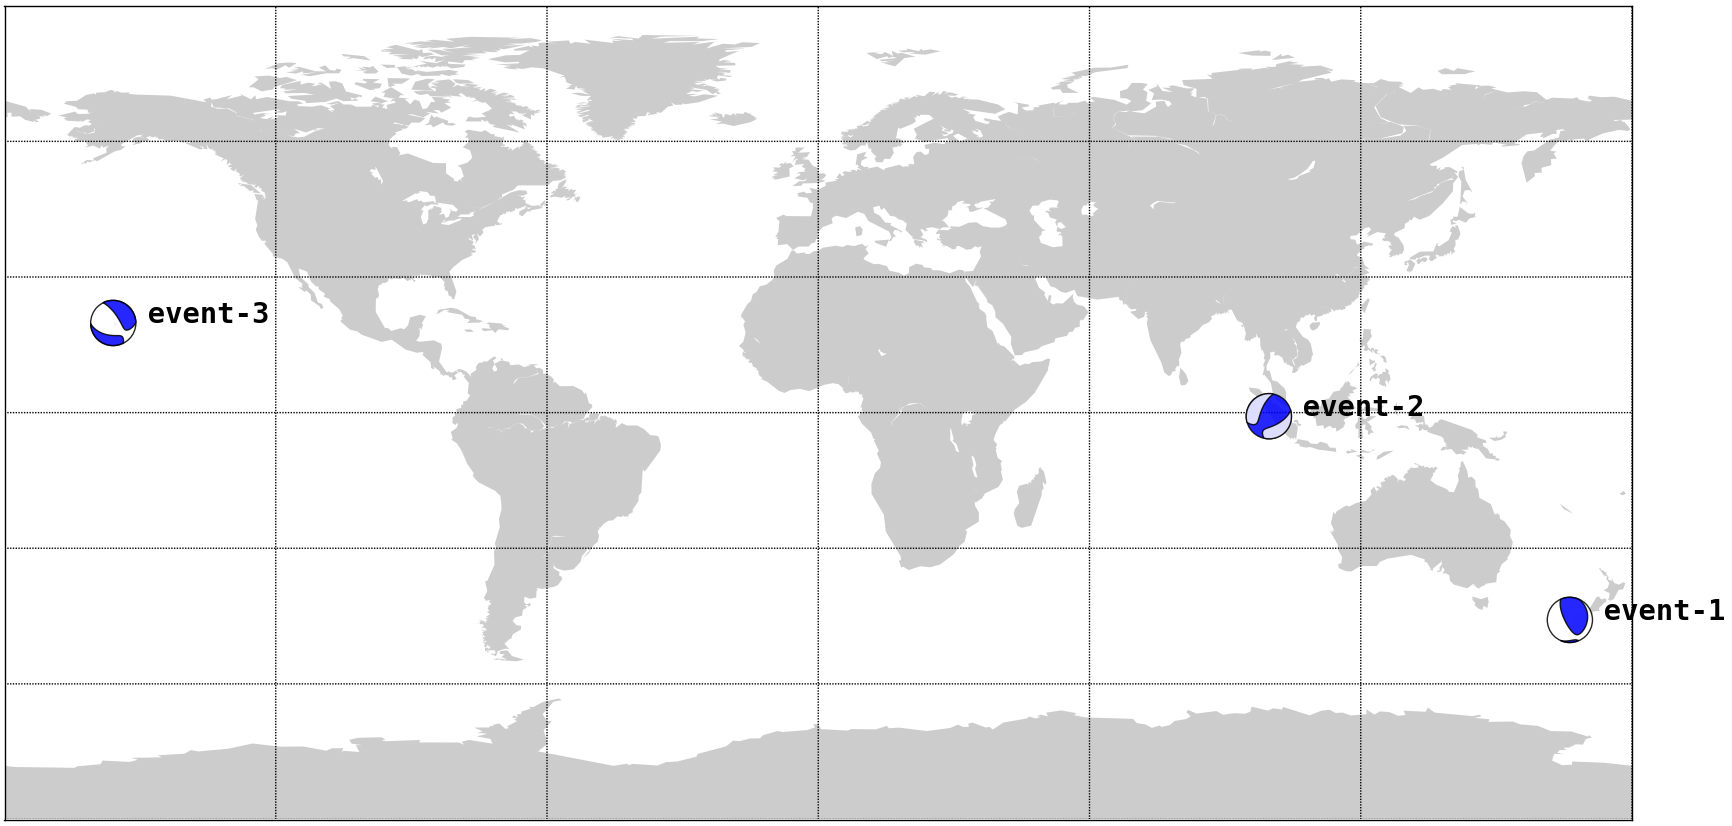
\includegraphics[width=372pt, height=178pt, keepaspectratio=true]{AXISEMTutorial-fig001.png}
%%\caption{This should be the caption for \texttt{AXISEMTutorial-fig001.png}.}
%%\end{figure}

{\small{}Figure A1: beach ball diagrams of event-1 to event-3 (based on GCMT catalog)}

\vspace{1cm}
%%\begin{figure}[htbp]
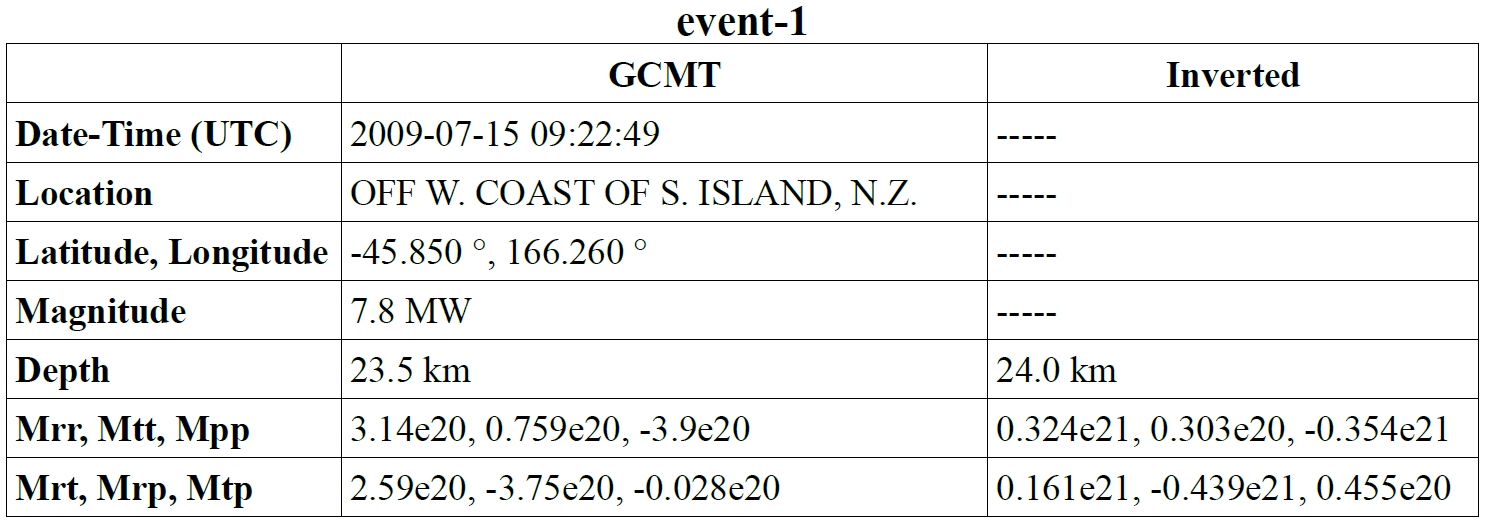
\includegraphics[width=312pt, height=110pt, keepaspectratio=true]{AXISEMTutorial-fig002.png}
%%\caption{This should be the caption for \texttt{AXISEMTutorial-fig002.png}.}
%%\end{figure}

\vspace{1cm}
%%\begin{figure}[htbp]
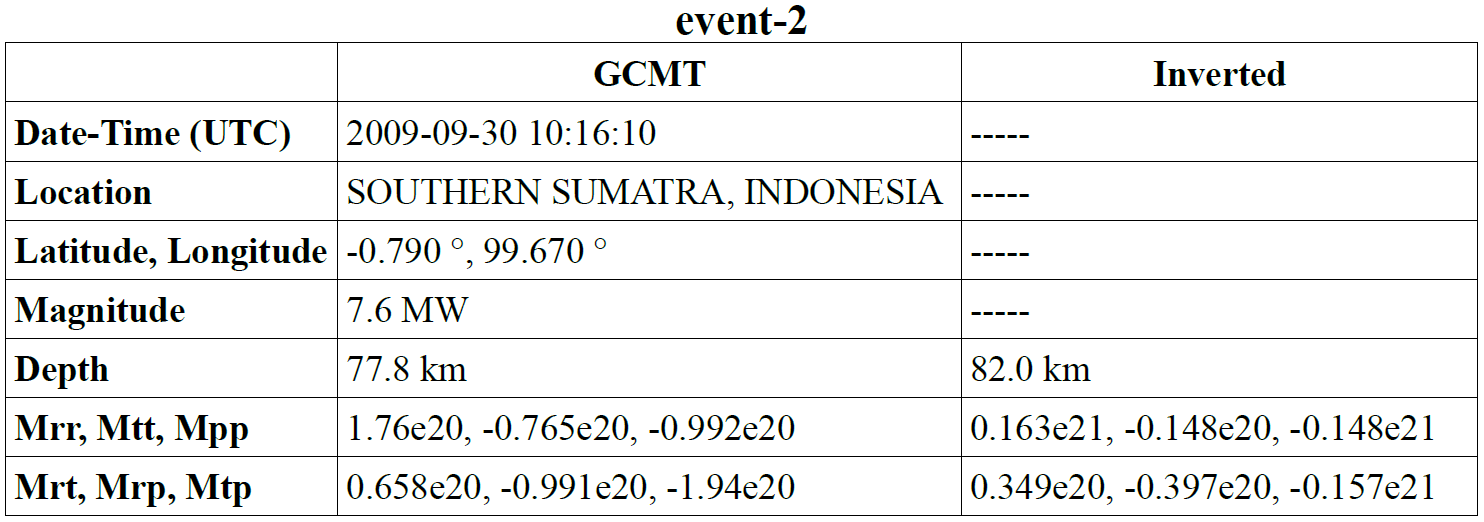
\includegraphics[width=312pt, height=110pt, keepaspectratio=true]{AXISEMTutorial-fig003.png}
%%\caption{This should be the caption for \texttt{AXISEMTutorial-fig003.png}.}
%%\end{figure}

\vspace{1cm}
%%\begin{figure}[htbp]
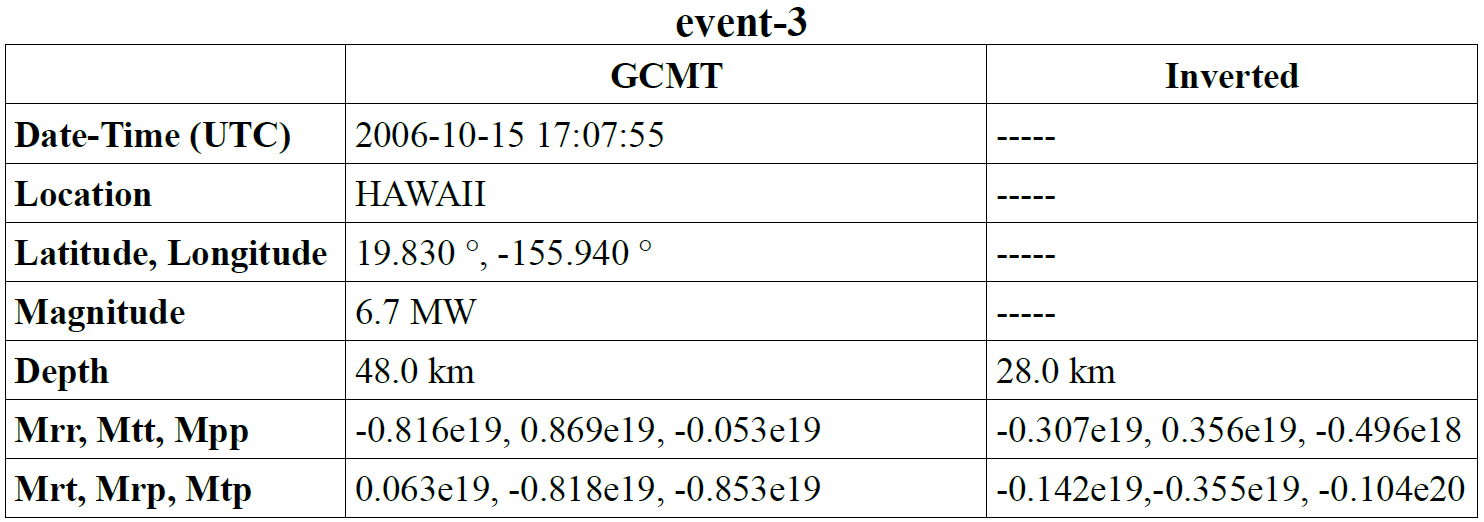
\includegraphics[width=312pt, height=110pt, keepaspectratio=true]{AXISEMTutorial-fig004.png}
%%\caption{This should be the caption for \texttt{AXISEMTutorial-fig004.png}.}
%%\end{figure}

\end{center}


%\baselineskip=13pt
%\leftskip=0pt

\newpage

\section{APPENDIX-2: Folder structure}

Figure A2 shows how the events (and their meta-data), waveforms and scripts are 
organized in the Virtual-box:

\begin{center}
%%\begin{figure}[htbp]
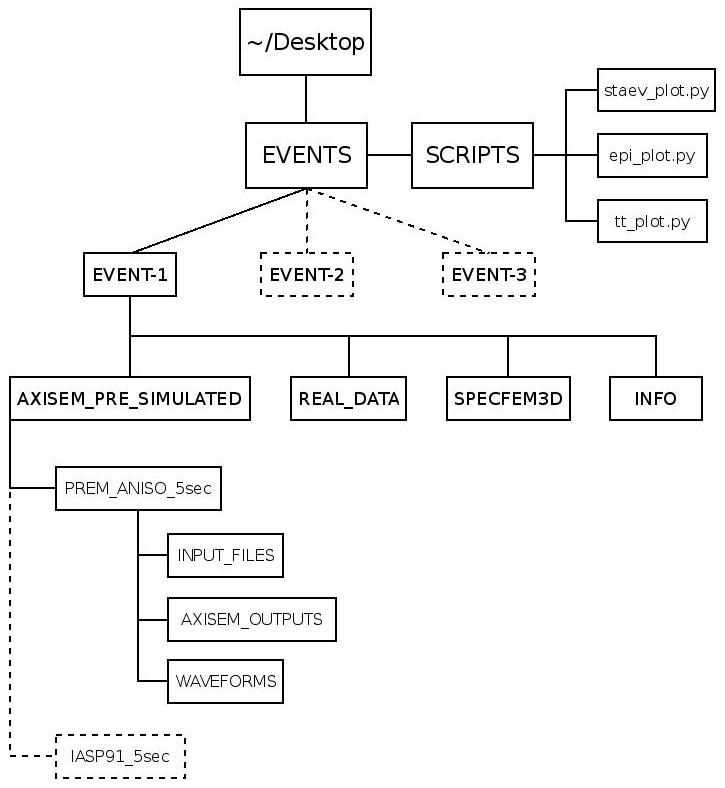
\includegraphics[width=334pt, height=362pt, keepaspectratio=true]{AXISEMTutorial-fig005.jpg}

Figure A2: Folder structure
%%\end{figure}
\end{center}

In \textit{SCRIPTS} directory, there are three python scripts that we use here:

\begin{enumerate}
    \item \textbf{plot\_station\_event\_distribution.py}: maps event and stations of an
    event directory.
    \item \textbf{plot\_seismograms.py}: plotting tool for comparison purposes.
    \item \textbf{plot\_travel\_time\_map.py}: project the time shift derived by cross
    correlating the AXISEM waveforms and real data.
\end{enumerate}

In \textit{EVENTS} directory, there are three events, each with the following
sub-directories:

\begin{enumerate}
    \item \textbf{AXISEM\_PRE\_SIMULATED}: contains seismograms simulated by AXISEM with
    the required input files to re-produce them.
    \item \textbf{REAL\_DATA}: seismograms retrieved from \textit{IRIS. }(refer to
    APPENDIX-5)
    \item \textbf{SPECFEM3D}: waveforms simulated by SPECFEM3D for comparison purposes 
    (downloaded from\textit{ IRIS}, refer to APPENDIX-5)
    \item \textbf{INFO}: information about the event and stations: event\_1.xml and
    STATIONS
\end{enumerate}


\newpage
\section{APPENDIX-3: A Quick Guide to PyAxi}

PyAxi is a Python script developed as an interface for AXISEM. All the options 
available in AXISEM are included in only one input file (inpython.cfg). By running 
the script, all the necessary steps (MESHER, SOLVER and Post-Processing) will be 
done automatically. \\

All you should do to run PyAxi for an input file (inpython.cfg) and station list 
(STATIONS) is:
\begin{verbatim}
    $ python PyAxi <inpython.cfg> <STATIONS>
\end{verbatim}

and the rest should be done automatically. inpython.cfg is a conguration file that 
contains all the AXISEM options. To change the input file, open inpython.cfg with 
an editor. However, you could find some already prepared inpython.cfg files for 
the events in Virtual-box. (refer to APPENDIX-2 for more information, Figure A2 
\textit{INPUT\_FILES}) Therefore, to run the AXISEM for the provided events (EVENT-1 
and IASP91-5sec as an example), it is enough to replace:

\begin{verbatim}
    <inpython.cfg>: 
    ~/Desktop/EVENTS/EVENT-1/AXISEM_PRE_SIMULATED/IASP91_5sec/INPUT_FILES/inpython.cfg
    
    <STATIONS>:
    ~/Desktop/EVENTS/EVENT-1/AXISEM_PRE_SIMULATED/IASP91_5sec/INPUT_FILES/STATIONS
\end{verbatim}

\newpage

\section{APPENDIX-4: Run AXISEM for EVENT-1}

In this appendix, we follow the steps in the main tutorial and show the commands 
and outcomes for each step. For this reason, we focus on one of the events, EVENT-1. \\

Start from within the \verb|Desktop/EVENTS| directory:

1. Plot one of the events (listed in EVENTS directory, we choose EVENT-1 in this example):
\begin{verbatim}
    $ plot_station_event_distribution.py EVENT-1
\end{verbatim}
* For more information on the folder structure of your Virtual-Box, refer to Appendix-2.

\begin{center}
%%\begin{figure}[htbp]
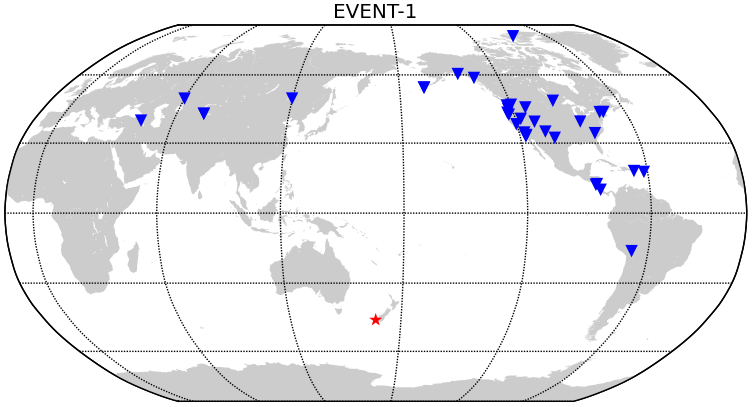
\includegraphics[width=444pt, height=240pt, keepaspectratio=true]{AXISEMTutorial-fig006.png}
%%\caption{This should be the caption for \texttt{AXISEMTutorial-fig006.png}.}
%%\end{figure}

{\small{}Figure A2: Event-station configuration for EVENT-1}
\end{center}

\baselineskip=13pt
\leftskip=0pt
2. To get an overview on both real data and pre-simulated seismograms: (e.g. PREM\_ANISO 
for 5 seconds dominant period) [Figure A3]
\begin{verbatim}
    $ plot_seismograms.py EVENT-1/AXISEM_PRE_SIMULATED/PREM_ANISO_5sec
\end{verbatim}

3.Cut the waveforms for Pdiff and PKiKP seismic phases and plot the seismograms: 
(compared with real data)
\begin{verbatim}
    $ plot_seismograms.py EVENT-1/AXISEM_PRE_SIMULATED/PREM_ANISO_5sec Pdiff
    $ plot_seismograms.py EVENT-1/AXISEM_PRE_SIMULATED/PREM_ANISO_5sec PKiKP
\end{verbatim}

\begin{figure}
%%\begin{figure}[htbp]
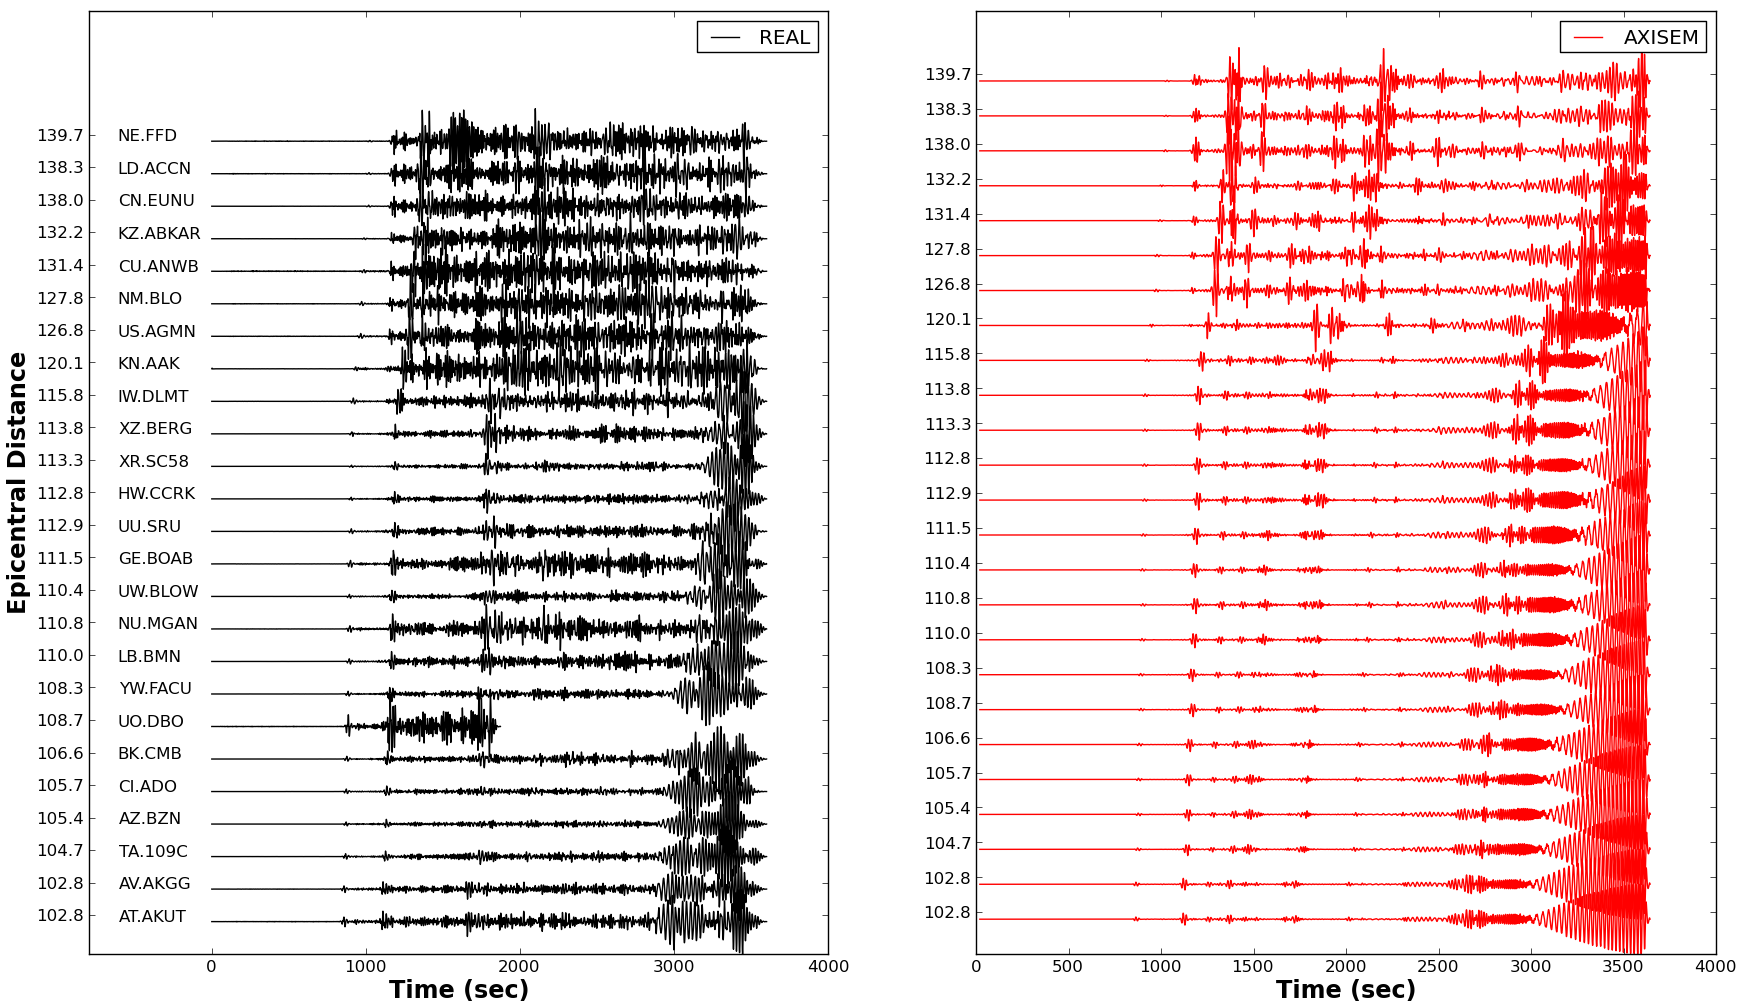
\includegraphics[width=497pt, height=287pt, keepaspectratio=true]{AXISEMTutorial-fig007.png}
%%\caption{This should be the caption for \texttt{AXISEMTutorial-fig007.png}.}
%%\end{figure}
\begin{center}
{\small{}Figure A3:Real and AXISEM waveforms for EVENT-1}
\end{center}
\end{figure}

\begin{figure}
\centering
\begin{minipage}{.5\textwidth}
  \centering
  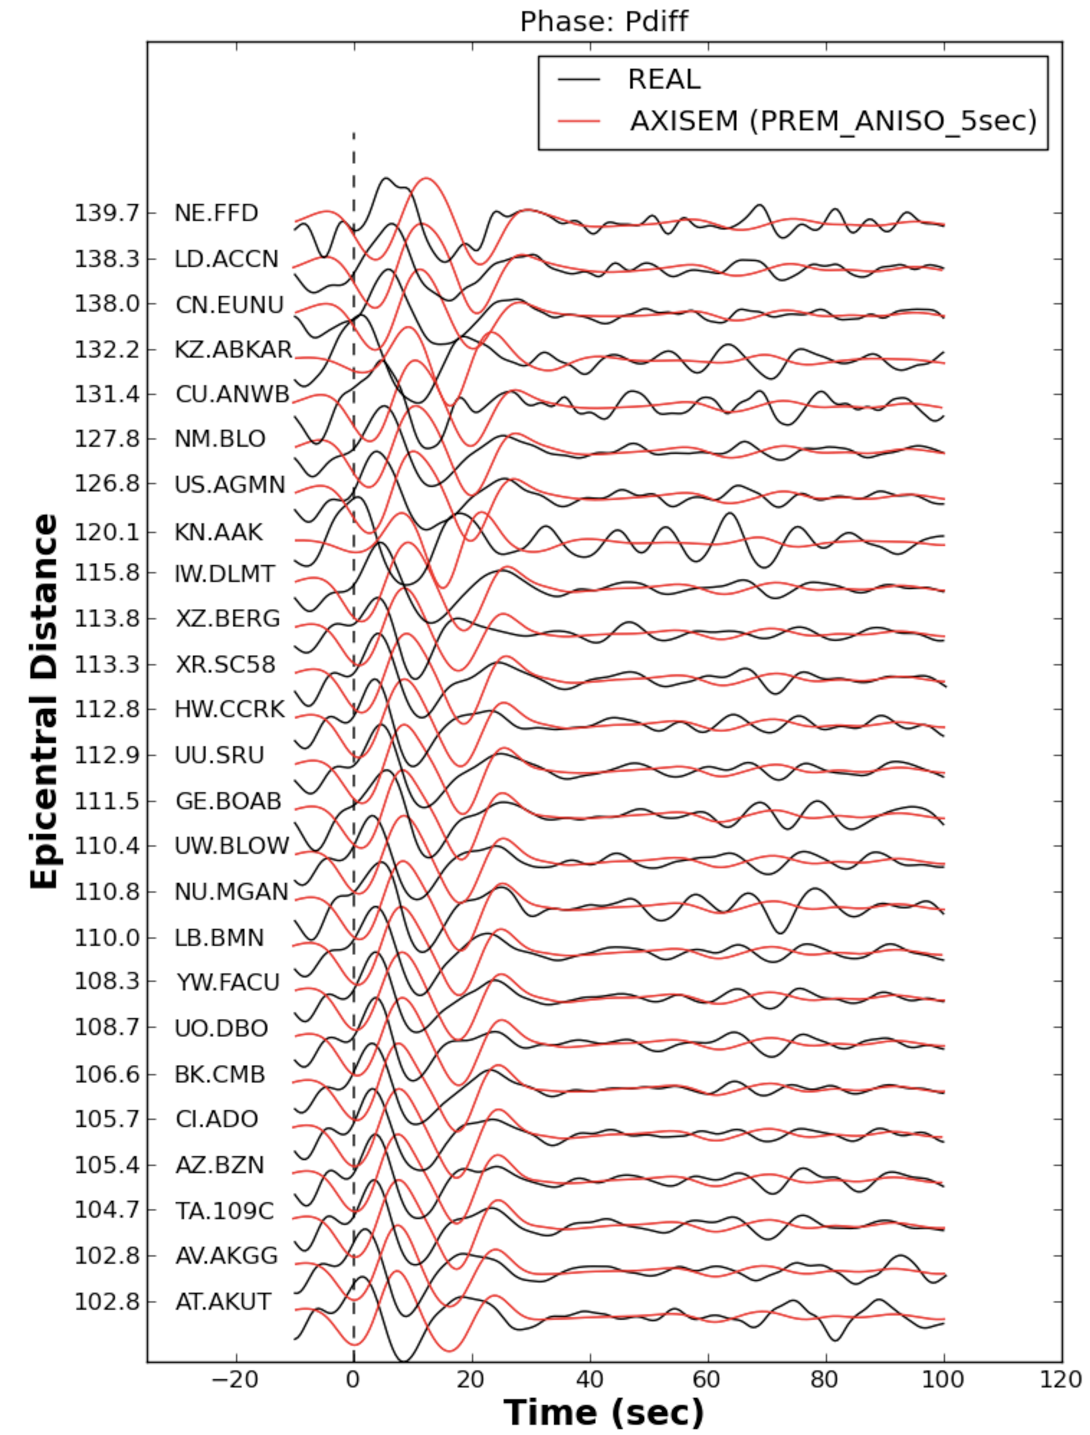
\includegraphics[width=1.\linewidth]{AXISEMTutorial-fig008.pdf}
  %\includegraphics[width=.4\linewidth]{image1}
\end{minipage}%
\begin{minipage}{.5\textwidth}
  \centering
  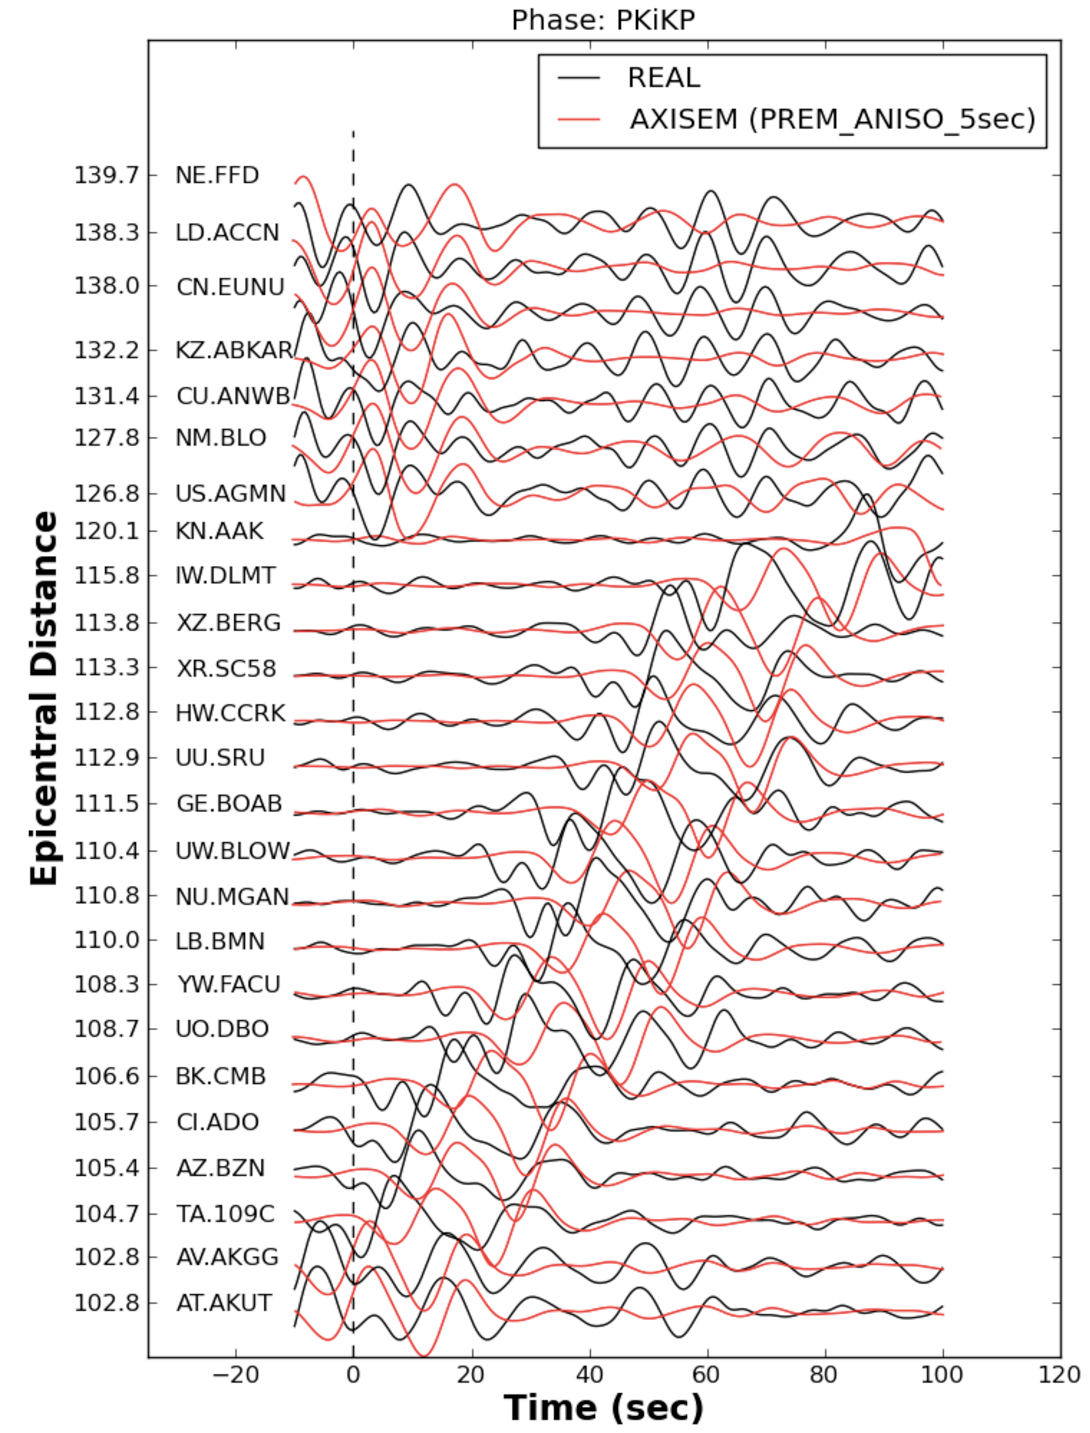
\includegraphics[width=1.\linewidth]{AXISEMTutorial-fig009.pdf}
%   \includegraphics[width=.4\linewidth]{image1}
\end{minipage}
\begin{center}
{\small{}Figure A4: Comparison between real and synthetic waveforms for Pdiff and 
PKiKP phases.}
\end{center}
\end{figure}


4. Change the filter in \textit{plot\_seismograms.py} script and compare the results with 
\textit{SPECFEM3D}: (for changing the filter, open \textit{plot\_seismograms.py} and change 
values at top of the file) \\
For this example, ????? we change hfreq (high frequency) in line 34 to 0.05Hz (20sec) and \textit{lfreq }to 0.01Hz: (Figure 
A5)

\begin{verbatim}
    $ plot_seismograms.py EVENT-1/AXISEM_PRE_SIMULATED/PREM_ANISO_5sec Pdiff specfem3d
    $ plot_seismograms.py EVENT-1/AXISEM_PRE_SIMULATED/PREM_ANISO_5sec PKiKP specfem3d
\end{verbatim}


\begin{figure}
\centering
\begin{minipage}{.5\textwidth}
  \centering
  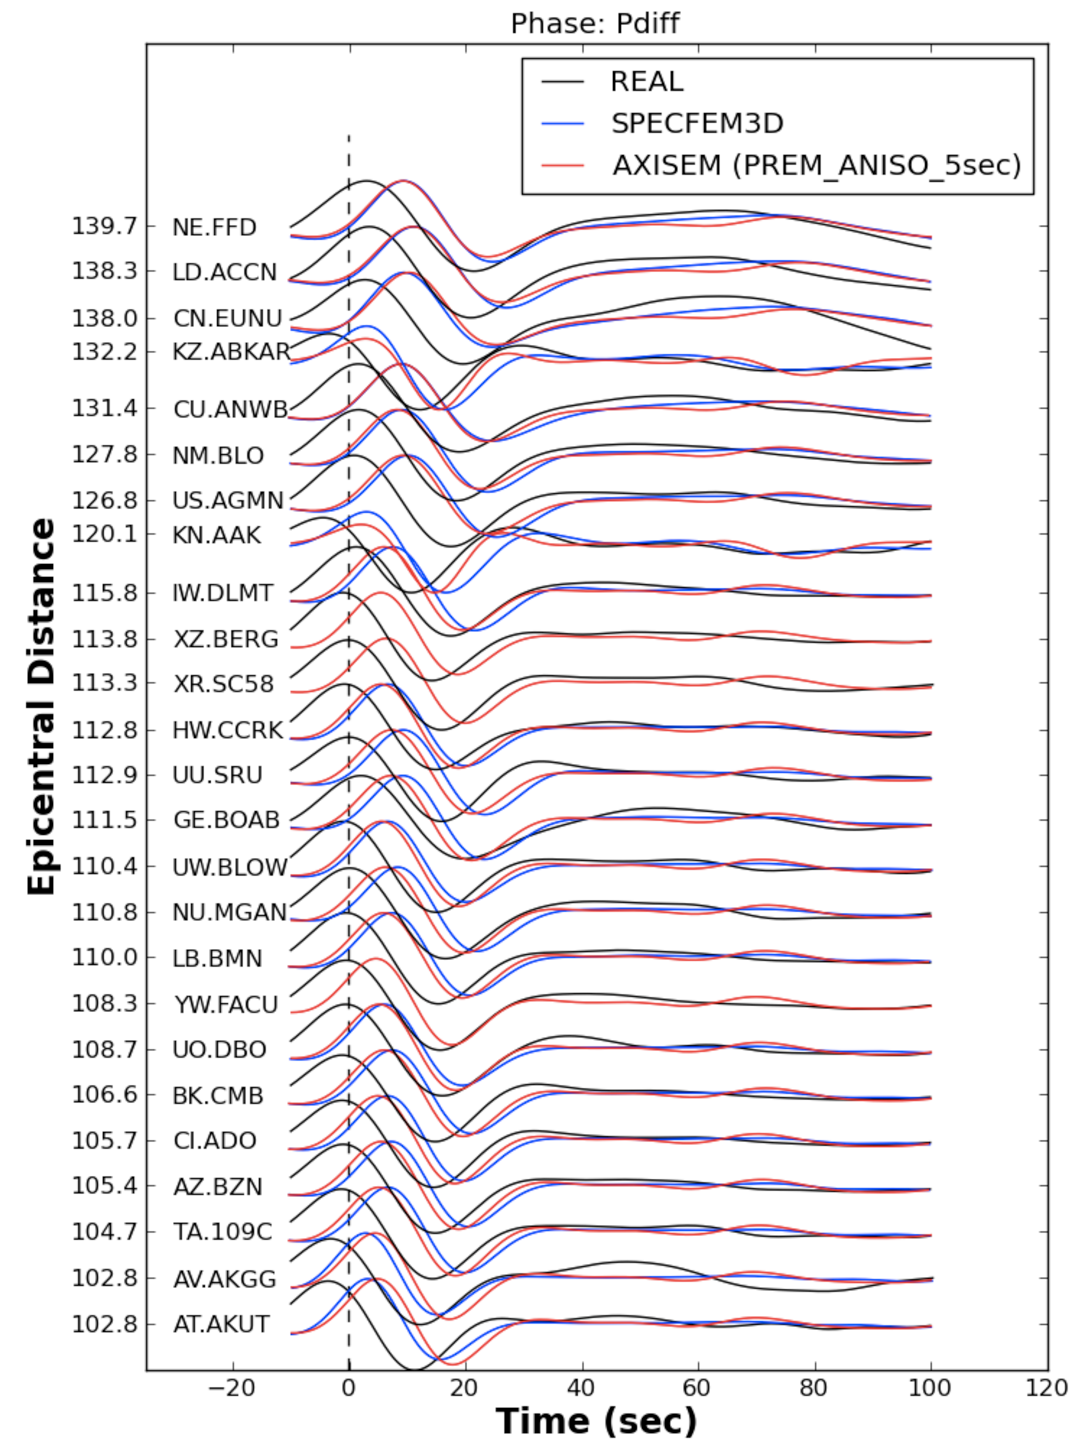
\includegraphics[width=1.\linewidth]{AXISEMTutorial-fig010.pdf}
  %\includegraphics[width=.4\linewidth]{image1}
\end{minipage}%
\begin{minipage}{.5\textwidth}
  \centering
  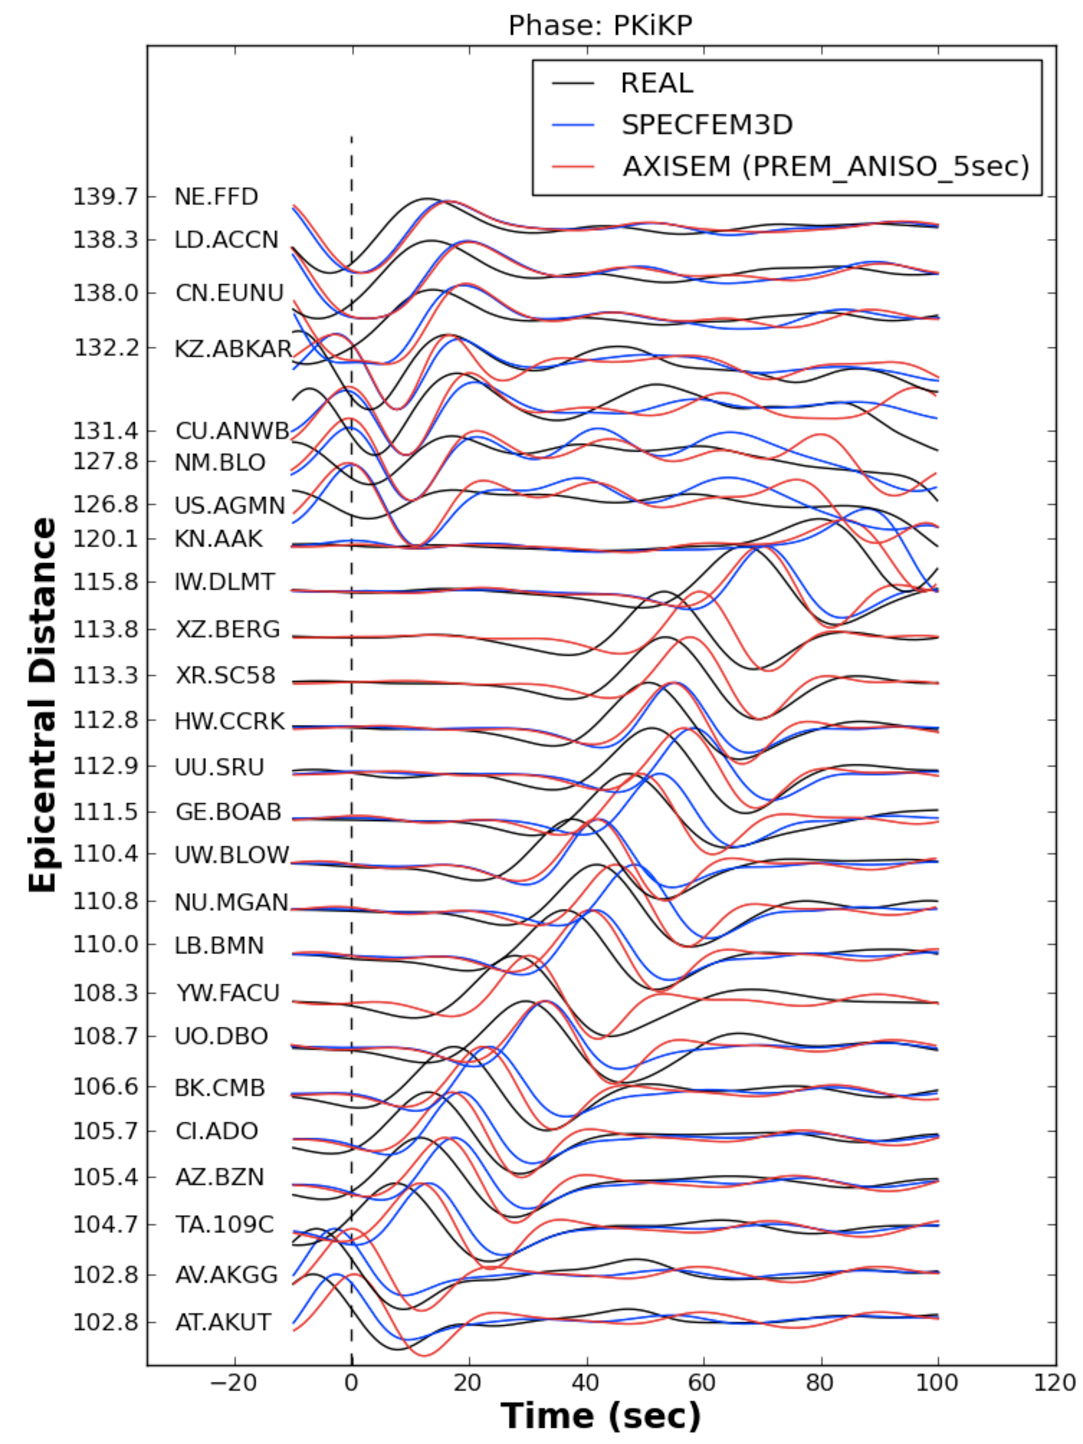
\includegraphics[width=1.\linewidth]{AXISEMTutorial-fig011.pdf}
%   \includegraphics[width=.4\linewidth]{image1}
\end{minipage}
\begin{center}
{\small{}Figure A5: Comparison between real, AXISEM and SPECFEM3D waveforms for 
Pdiff and PKiKP phases.}
\end{center}
\end{figure}

5. Compare the results of two different background models (\textit{PREM\_ANISO\_5sec} with 
\textit{IASP91\_5sec)} for Pdiff phase: (Figure A6).

\begin{verbatim}
    $ plot_seismograms.py EVENT-1/AXISEM_PRE_SIMULATED/PREM_ANISO_5sec Pdiff 
    EVENT-1/AXISEM_PRE_SIMULATED/IASP91_5sec
\end{verbatim}

6. Change the filter, as explained in step 4, and repeat step 5. Here, we increase 
the \textit{hfreq} to 0.2Hz and \textit{lfreq} to 0.05Hz (Figure A7).

\begin{figure}
\centering
%%\begin{figure}[htbp]
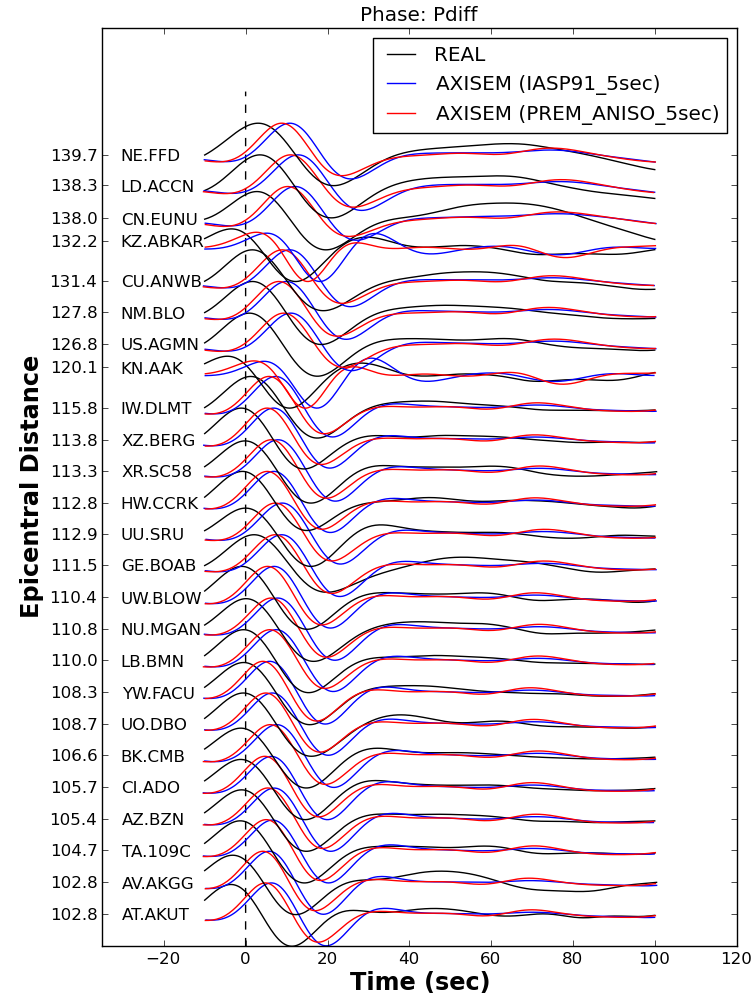
\includegraphics[width=234pt, height=310pt, keepaspectratio=true]{AXISEMTutorial-fig012.png}
\begin{center}
{\small{}Figure A6: Comparison between real and AXISEM waveforms for two different 
background models (Pdiff).}
\end{center}
\end{figure}

\begin{figure}
\centering
%%\begin{figure}[htbp]
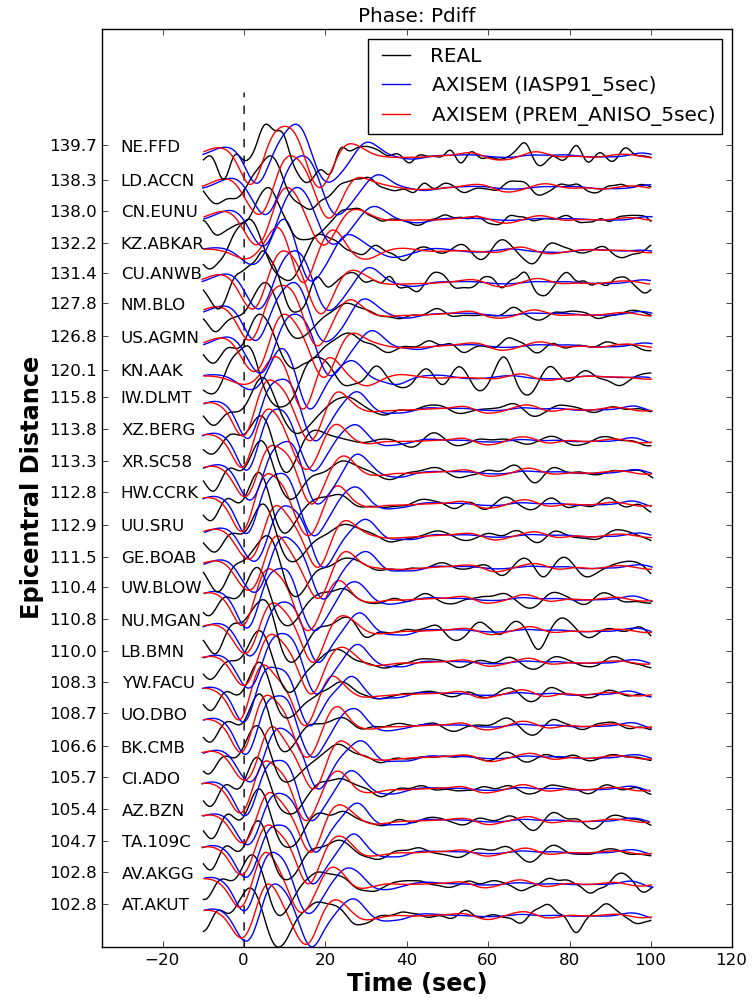
\includegraphics[width=241pt, height=320pt, keepaspectratio=true]{AXISEMTutorial-fig013.png}
\begin{center}
{\small{}Figure A7: Comparison between real and AXISEM waveforms for two different 
background models (Pdiff).} 
\end{center}
\end{figure}

7. Compare the seismograms calculated for two different source parameters (PREM\_ANISO\_5sec and \\
PREM\_ANSIO\_5sec\_GCMT) for Pdiff phase: (For more information about the source 
parameters, refer to Appendix-1) [Figure A8]

\begin{verbatim}
    $ plot_seismograms.py EVENT-1/AXISEM_PRE_SIMULATED/PREM_ANISO_5sec Pdiff 
    EVENT-1/AXISEM_PRE_SIMULATED/PREM_ANISO_5sec_GCMT
\end{verbatim}

\begin{figure}
\centering
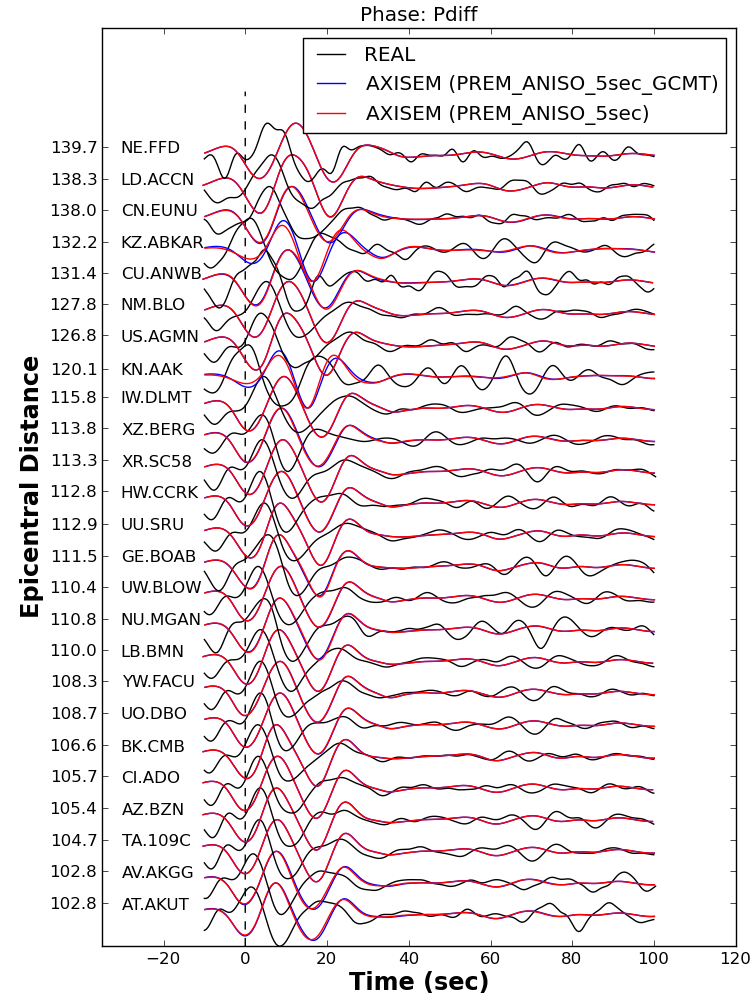
\includegraphics[width=234pt, height=310pt, keepaspectratio=true]{AXISEMTutorial-fig014.png}
\begin{center}
{\small{}Figure A8: Comparison between real and AXISEM waveforms for two different 
source parameters (Pdiff).}
\end{center}
\end{figure}

8. Change the filter, as explained in step 4, and repeat step 7. ????? Here, we decrease 
the \textit{hfreq} to 0.05Hz and \textit{lfreq} to 0.01Hz. (Figure A9)

9. Find the time shift between the synthetics and real data, shift the synthetics 
accordingly and plot the results: (Figure A10)

\begin{verbatim}
    $ plot_seismograms.py EVENT-1/AXISEM_PRE_SIMULATED/PREM_ANISO_5sec Pdiff shift_synthetics
\end{verbatim}

\vspace{13pt}
10. Map the calculated time shifts in step 9 on the station locations: (note that 
it always plots the results of the latest comparison, i.e. Pdiff here) 

\begin{verbatim}
    $ plot_travel_time_map.py EVENT-1
\end{verbatim}

\begin{center}
%%\begin{figure}[htbp]
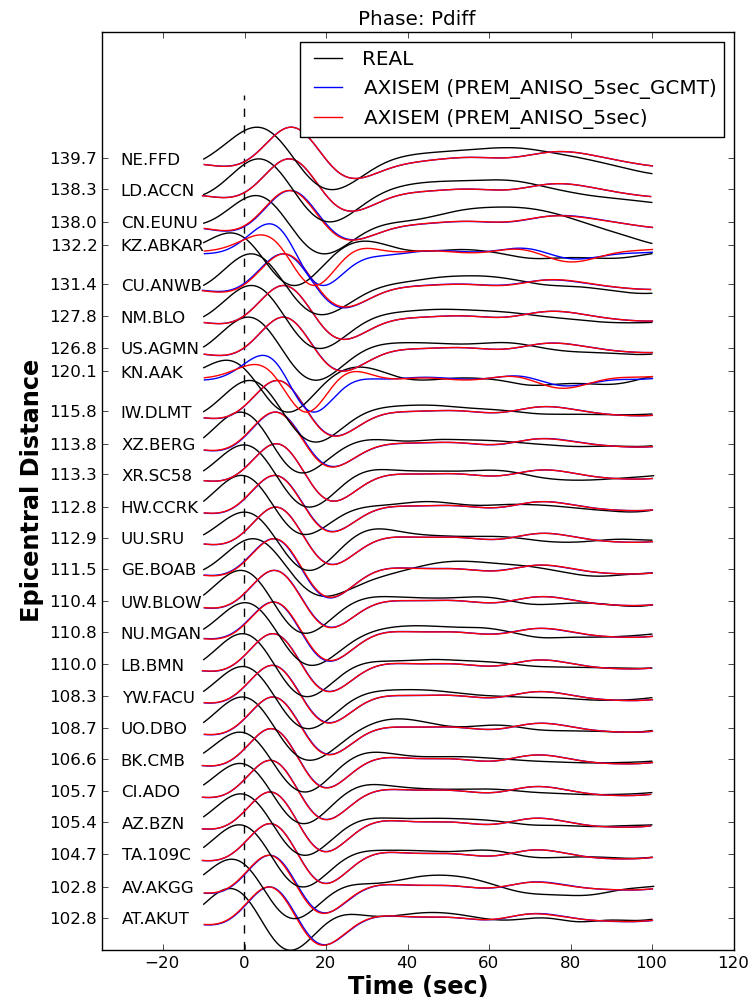
\includegraphics[width=242pt, height=322pt, keepaspectratio=true]{AXISEMTutorial-fig015.png}
%%\caption{This should be the caption for \texttt{AXISEMTutorial-fig015.png}.}
%%\end{figure}

{\small{}Figure A9: Comparison between real and AXISEM waveforms for two different 
source parameters (Pdiff).}

%%\begin{figure}[htbp]
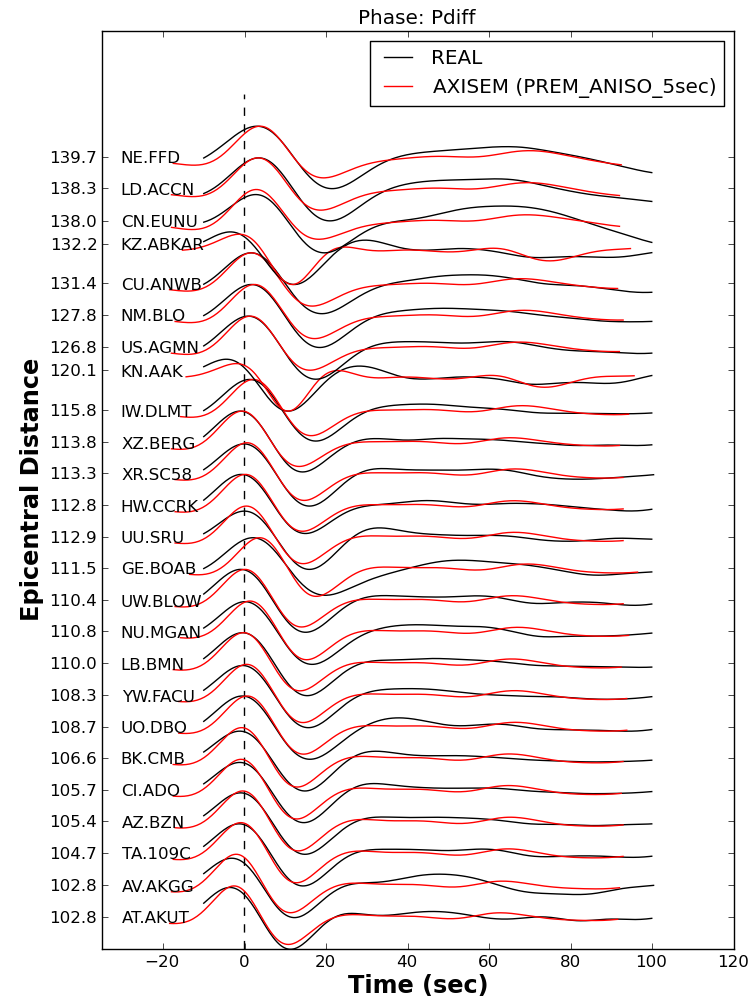
\includegraphics[width=249pt, height=331pt, keepaspectratio=true]{AXISEMTutorial-fig016.png}
%%\caption{This should be the caption for \texttt{AXISEMTutorial-fig016.png}.}
%%\end{figure}

{\small{}Figure A10: Comparison between real and AXISEM waveforms for Pdiff. AXISEM 
waveforms are shifted in order to gain the maximum cross correlation coefficient.}

\vspace{1cm}

%%\begin{figure}[htbp]
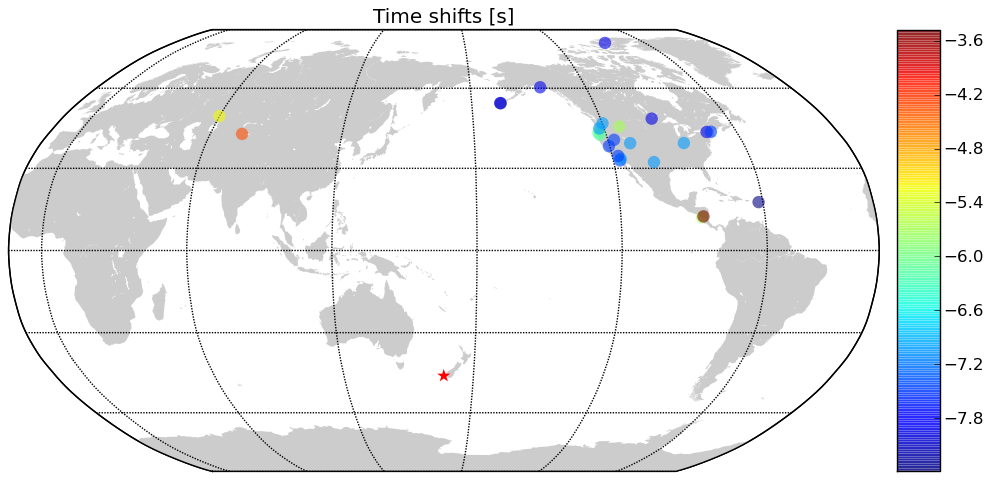
\includegraphics[width=446pt, height=217pt, keepaspectratio=true]{AXISEMTutorial-fig017.png}
%%\caption{This should be the caption for \texttt{AXISEMTutorial-fig017.png}.}
%%\end{figure}

{\small{}Figure A11: Time shift calculated by cross correlation between real and 
AXISEM waveforns. Blue color indicates that Pdiff in real data arrived sooner than 
that in the synthetic one.}
\end{center}

\baselineskip=13pt
\leftskip=0pt

\newpage
\section{APPENDIX-5: Retrieving real data and SPECFEM3D seismograms automatically}

{\color{color18} \emph{obspyDMT}} (ObsPy Data Management Tool) is a command line 
tool for retrieving, processing and management of massive seismological data in 
a fully automatic way which could be run in serial or in parallel. \\

This tool is developed to mainly address the following tasks automatically:

1. Retrieval of waveforms (MSEED or SAC), response files and metadata from {\color{color18} \emph{IRIS}} 
and {\color{color18} \emph{ORFEUS}} (via {\color{color18} \emph{ArcLink}}) archives. 
This could be done in \textit{serial} or in \textit{parallel} for single or large 
requests.

2. Supports event-based and continuous requests.

3. Extracting the information of all the events via user-defined options (time 
span, magnitude, depth and event location) from {\color{color18} \emph{IRIS}} and 
{\color{color18} \emph{EMSC}} (European Mediterranean Seismological Centre).

4. Updating the existing archives (waveforms, response files and metadata).

5. Processing the data in \textit{serial} or in \textit{parallel} (e.g. \textit{Tapering, 
removing the trend of the time series, filtering and Instrument correction}).

6. Management of large seismic datasets.

7. Plotting tools (events and/or station locations, Ray coverage (event-station 
pair), epicentral-distance plots for all archived waveforms and seismicity maps).

\vspace{13pt}
Here, we use obspyDMT to retrieve both real data and SPECFEM3D seismograms. For 
more information about this tool please refer to the following webpage:

{\color{color18} \emph{https://github.com/kasra-hosseini/obspyDMT}}  \\

obspyDMT is installed on your virtual machine. By running the following commands, 
the real data used in this tutorial can be retrieved automatically:

\textbf{Event-1:}

\begin{verbatim}
    ./obspyDMT.py --datapath EVENT-1_real --min_date 2009-07-15 --max_date 2009-07-16 
    --min_mag 7.0 --min_depth 20 --list_stas ~/Desktop/EVENT-1/INFO/STATIONS 
    --offset 3600 --req_parallel --arc N
\end{verbatim}

\textbf{Event-2:}

\begin{verbatim}
    ./obspyDMT.py --datapath EVENT-2_real --min_date 2009-09-30 --max_date 2009-10-01 
    --min_mag 7.0 --min_depth 70 --list_stas ~/Desktop/EVENT-1/INFO/STATIONS 
    --offset 3600 --req_parallel --arc N
\end{verbatim}

\textbf{Event-3:}

\begin{verbatim}
    ./obspyDMT.py --datapath EVENT-3_real --min_date 2006-10-15 --max_date 2006-10-16 
    --min_mag 6.0 --min_depth 20 --list_stas ~/Desktop/EVENT-1/INFO/STATIONS 
    --offset 3600 --req_parallel --arc N
\end{verbatim}

Moreover, the SPECFEM3D seismograms can be also retrieved in the same manner:

\textbf{Event-1:}

\begin{verbatim}
    ./obspyDMT.py --datapath EVENT-1 --min_date 2009-07-15 --max_date 2009-07-16 
    --min_mag 7.0 --min_depth 20 --list_stas ~/Desktop/EVENT-1/INFO/STATIONS 
    --specfem3D --offset 3600 --req_parallel --arc N
\end{verbatim}

\textbf{Event-2:}

\begin{verbatim}
    ./obspyDMT.py --datapath EVENT-2 --min_date 2009-09-30 --max_date 2009-10-01 
    --min_mag 7.0 --min_depth 70 --list_stas ~/Desktop/EVENT-1/INFO/STATIONS 
    --specfem3D --offset 3600 --req_parallel --arc N
\end{verbatim}

\textbf{Event-3:}

\begin{verbatim}
    ./obspyDMT.py --datapath EVENT-3 --min_date 2006-10-15 --max_date 2006-10-16 
    --min_mag 6.0 --min_depth 20 --list_stas ~/Desktop/EVENT-1/INFO/STATIONS 
    --specfem3D --offset 3600 --req_parallel --arc N
\end{verbatim}

\end{document}
